\section{Data and Exploratory Analysis}
\label{sec:data}

% TODO (group writes the text). Cover:
% - Sources: ENEM 2025 microdata and School Census 2024 (INEP); include the DATASET DOWNLOAD LINK
%   (required by the assignment). URLs and SHA-256 of each source are in the metadata JSON
%   generated by scripts/build_dataset.py (data/processed/*.json).
% - Unit of analysis: school with >= 10 candidates present in all 4 tests; target nota_media
%   (mean over schools of the mean of the 5 scores). Number of schools and attributes (README.md).
% - EDA findings required by the assignment: attribute types/quantity, target distribution,
%   patterns, anomalies (88888 code, 15 schools), missing values, scale, outliers, inconsistencies.
%   Source: ../reports/eda.md.
% - Figures below: choose which to keep (page limit is 20 pages including references).

\subsection{Sources and construction of the data set}

Two public data sets published by INEP were used: the ENEM 2025 microdata
\cite{inep2025enem}, file \texttt{RESULTADOS\_2025.csv}, available at
\url{https://download.inep.gov.br/microdados/microdados_enem_2025.zip}, and the Censo Escolar
2024 microdata \cite{inep2024censo}, available at
\url{https://download.inep.gov.br/dados_abertos/microdados_censo_escolar_2024.zip}. The 2024
census was selected because the 2025 edition had not been published when the data were collected; the
structural characteristics of a school change slowly, so the one-year lag should have little
effect, but we return to it in Section~\ref{sec:conclusion}.

A candidate is kept only if present in the four ENEM tests, with the five scores (natural
sciences, human sciences, languages, mathematics, and essay) and a school code. This leaves
1{,}288{,}485 candidates in 29{,}341 schools. For each candidate we take the mean of the five
scores, and for each school the mean over its candidates; this school mean, \texttt{nota\_media},
is the target. We keep schools with at least ten valid candidates (23{,}570 schools), so that the
target is not dominated by a handful of students, and join them with the census by school code.
The final table has \textbf{23{,}374 schools} (99.2\% of the schools above the threshold) in
5{,}201 municipalities.

Each school is described by 45 attributes from the census, chosen to represent what a school or
an education department can act upon: 31 binary infrastructure indicators (\texttt{IN\_*}, e.g.,
science laboratory, library, internet for students, school meals), 9 counts of size and resources
(\texttt{QT\_*}, e.g., high-school enrolment, teachers, rooms, computers), and 5 categorical
attributes of network and location (administrative network \texttt{TP\_DEPENDENCIA}, urban/rural
location, differentiated location, region, and state). The municipality code is used only to
define the cross-validation groups (Section~\ref{sec:methodology}) and is never a model input.


\begin{figure}[ht]
  \centering
  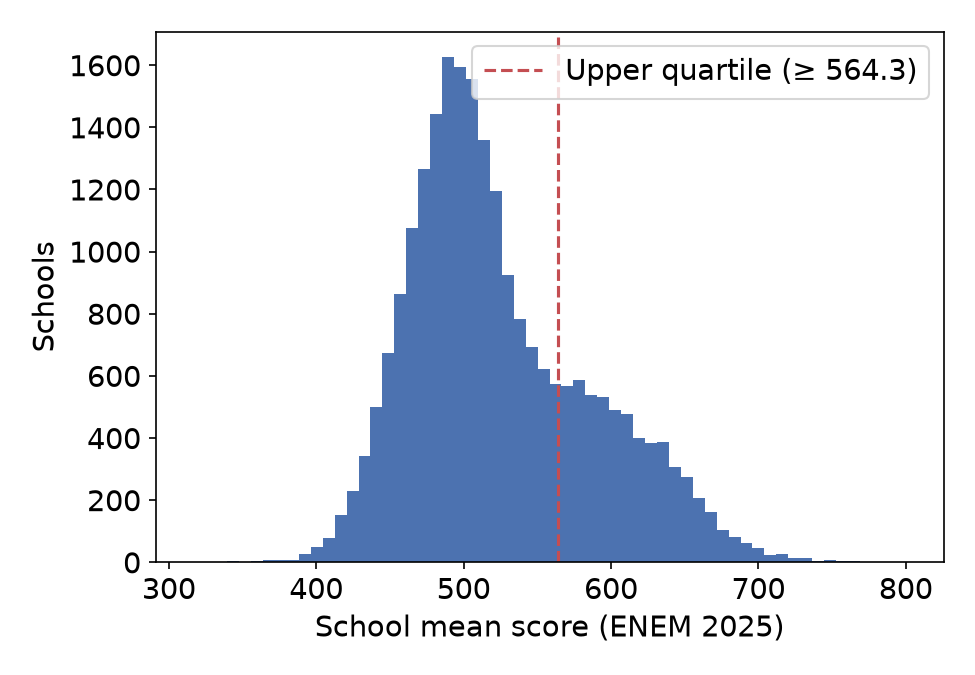
\includegraphics[width=0.7\textwidth]{target_hist.png}
  \caption{TODO: caption -- distribution of the target (\texttt{nota\_media}).}
  \label{fig:target-hist}
\end{figure}

\begin{figure}[ht]
  \centering
  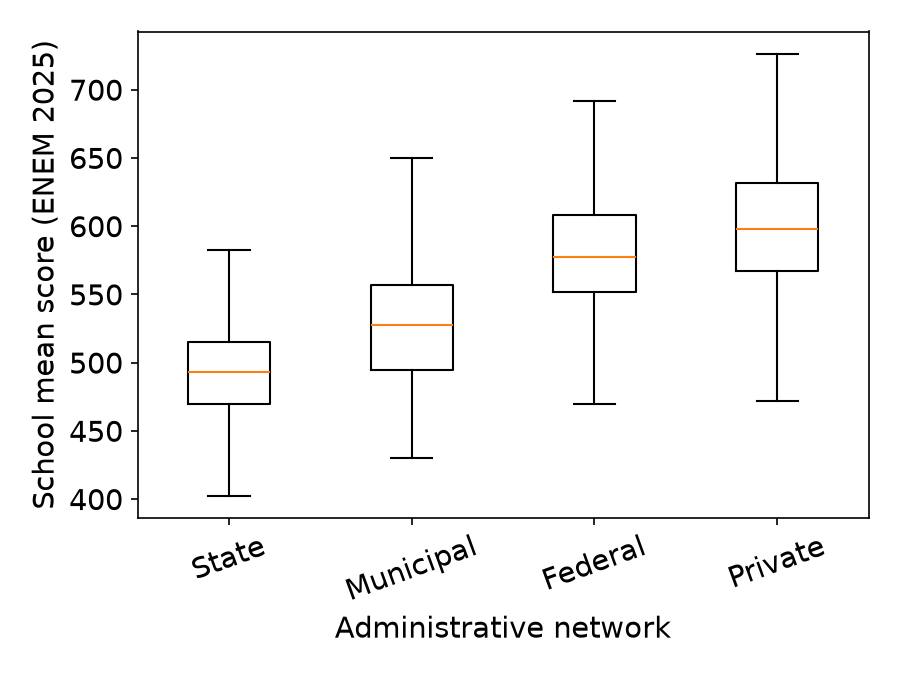
\includegraphics[width=0.7\textwidth]{target_by_dependencia.png}
  \caption{TODO: caption -- target by administrative network.}
  \label{fig:target-dependencia}
\end{figure}

\begin{figure}[ht]
  \centering
  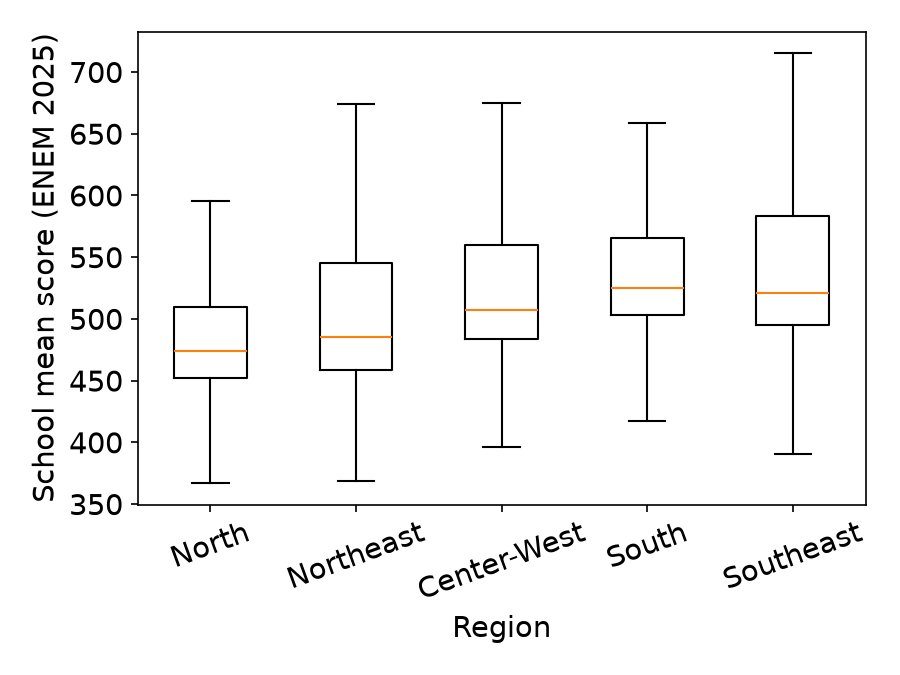
\includegraphics[width=0.7\textwidth]{target_by_regiao.png}
  \caption{TODO: caption -- target by region.}
  \label{fig:target-regiao}
\end{figure}

% Optional figures available in ../reports/figures/: feature_target_spearman.png,
% count_features_hist.png, target_std_by_school_size.png.
